\documentclass[10pt]{standalone}
\usepackage{stix}
\usepackage{tikz}
\usepackage{xcolor}
\usepackage{amsmath}
\usepackage{braket}
\usepackage{comment}
\definecolor{Fblue}{HTML}{560dcb}
\definecolor{Fred}{HTML}{92235a}
\definecolor{Firebrick}{HTML}{b22222}
\definecolor{Fnavy}{HTML}{000080}
\definecolor{ForangeRed}{HTML}{ff4500}
\definecolor{Fcornflower}{HTML}{bbddff}
\definecolor{Fcmix}{HTML}{0f4880}
\definecolor{Faqua}{HTML}{5fbf9f}
\definecolor{Fmagnifying}{HTML}{303030}
\newcommand{\bvec}[1]{\boldsymbol{#1}}
\usetikzlibrary{calc, arrows, arrows.meta, math} %, fpu}

\newcommand{\xp}[1]{\texttt{\color{ForangeRed}#1}}
\newcommand{\tp}[1]{\texttt{\color{Firebrick}#1}}
\newcommand{\tpd}[1]{\tp{#1} [displ,size]}
\newcommand{\ipd}[1]{#1 [displ, size]}

\newcommand{\bracketOne}[2]{
  \draw (cell#1.west) -- ++(-0.1,0.0) node {#2};
}
\newcommand{\bracketOneC}[2]{
  \draw (cell#1.west) -- ++(-0.05,0.0) node {#2};
}
\newcommand{\bracketOneS}[2]{
  \draw (cell#1.west) -- ++(-0.15,0.0) node {#2};
}
\newcommand{\bracketTwo}[3]{
  \tikzmath{\coordA = 0.5*(cell#1.west) + 0.5*(cell#2.west) + (-0.1,0.0);}
  \draw (cell#1.west) -- (\coordA);
  \draw (cell#2.west) -- (\coordA) node {#3};
}
\newcommand{\bracketThree}[4]{
  \tikzmath{\dbuf = 1./3.;
    \coordA = \dbuf*(cell#1.west) + \dbuf*(cell#2.west) + \dbuf*(cell#3.west) + (-0.1,0.0);}
  \draw (cell#1.west) -- (\coordA);
  \draw (cell#2.west) -- (\coordA);
  \draw (cell#3.west) -- (\coordA) node {#4};
}

\newcommand{\EbracketOne}[2]{
  \draw (Ecell#1.east) -- ++(0.1,0.0) node[anchor=west] {#2};
}
\newcommand{\EbracketTwo}[3]{
  \tikzmath{\coordA = 0.5*(Ecell#1.east) + 0.5*(Ecell#2.east) + (0.1,0.0);}
  \draw (Ecell#1.east) -- (\coordA);
  \draw (Ecell#2.east) -- (\coordA) node[anchor=west] {#3};
}
\newcommand{\EbracketThree}[4]{
  \tikzmath{\dbuf = 1./3.;
    \coordA = \dbuf*(Ecell#1.east) + \dbuf*(Ecell#2.east) + \dbuf*(Ecell#3.east) + (0.1,0.0);}
  \draw (Ecell#1.east) -- (\coordA);
  \draw (Ecell#2.east) -- (\coordA);
  \draw (Ecell#3.east) -- (\coordA) node[anchor=west] {#4};
}

\newcommand{\colorizeBox}[3]{
  \tikzmath{\coordA = (0,1-#1/64.0);
            \coordB = (1,1-#2/64.0);}
  \fill[draw=none, fill=#3] (\coordA) rectangle (\coordB);
}
\newcommand{\EcolorizeBox}[3]{
  \tikzmath{\coordA = (0,1-#1/64.0+67/64.0);
            \coordB = (1,1-#2/64.0+67/64.0);}
  \fill[draw=none, fill=#3] (\coordA) rectangle (\coordB);
}

\begin{document}
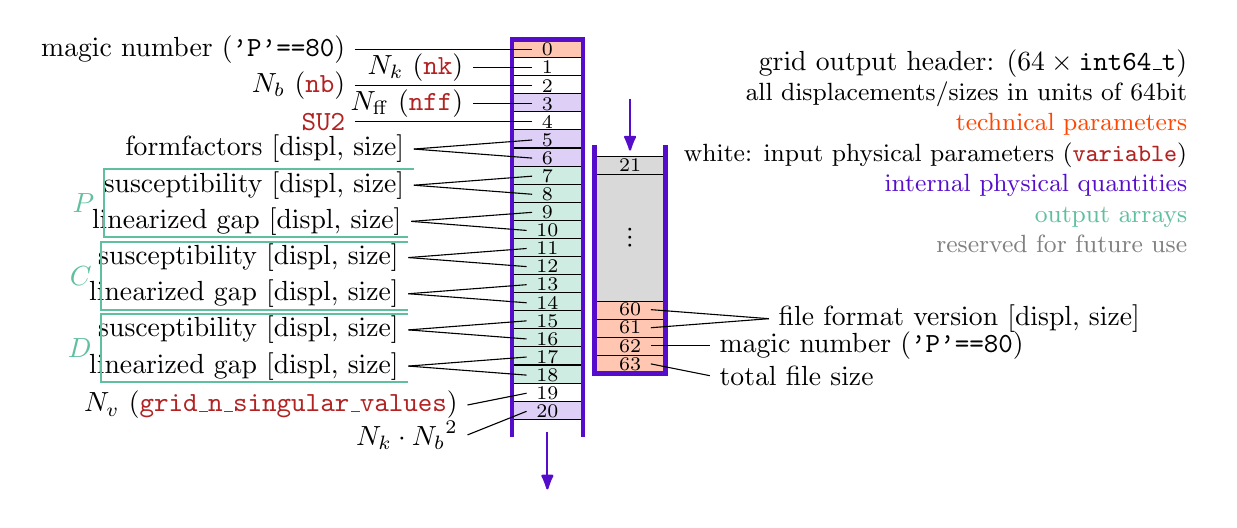
\begin{tikzpicture}[x=5.90552in, y=5.90552in, >={Latex[round]}]
  \clip (0,0.60) rectangle (1,1.0);
  \tikzmath{
    coordinate \coordA;
    coordinate \coordB;
    int \ibuf;
    real \dbuf;
  }
  \node[anchor=north east] at (0.99,0.99) {\begin{minipage}{3in}%
    \begin{flushright}%
      grid output header: $(64 \times \texttt{int64\_t})$\\
      \small
      all displacements/sizes in units of 64bit \\
      \textcolor{ForangeRed}{technical parameters} \\
      white: input physical parameters (\tp{variable}) \\
      \textcolor{Fblue}{internal physical quantities} \\
      \textcolor{Faqua}{output arrays} \\
      \textcolor{gray}{reserved for future use}
    \end{flushright}
  \end{minipage}};

  \begin{scope}[shift={(0.41,0.01)}, yscale=0.98, xscale=0.06]
    \colorizeBox{0}{1}{ForangeRed!30!white}
    \colorizeBox{3}{4}{Fblue!20!white}
    \colorizeBox{5}{7}{Fblue!20!white}
    \colorizeBox{20}{21}{Fblue!20!white}
    \colorizeBox{7}{19}{Faqua!30!white}

    \foreach \idx in {1,2,...,21} {
      \tikzmath{
        \dbuf = 1./64.;
        \ibuf = \idx-1;
        \coordA = (0,1-\idx/64.0);
        \coordB = (1,1-\idx/64.0);
      }
      \draw (\coordA) -- node[midway, above, yshift=-0.29em] (cell\ibuf) {\scriptsize\ibuf} (\coordB);
    }
    \tikzmath{ \dbuf = 1. - 20./64. - 2./64.; }
    \draw[Fblue, ultra thick] (0,\dbuf) -- (0,1) -- (1,1) -- (1,\dbuf);
    \tikzmath{ \dbuf = \dbuf + 0.005; }
    \draw[Fblue, ->, thick] (0.5,\dbuf) -- ++(0,-0.05);
  \end{scope}
  \begin{scope}[shift={(0.48,-0.089)}, yscale=0.98, xscale=0.06]
    \EcolorizeBox{67}{75}{gray!30!white}

    \EcolorizeBox{75}{78}{ForangeRed!30!white}
    \EcolorizeBox{78}{79}{ForangeRed!30!white}

    \tikzmath{
      int \add;
      int \iloc;
      coordinate \ctmpOne;
      coordinate \ctmpTwo;
      for \idx in {0,1,...,4} {
        if \idx>0 then {
          \add = 59;
          \iloc = \idx + 7;
        } else {
          \add = 21;
          \iloc = \idx + 0;
        };
        \ibuf = \add + \idx;
        \coordA = (0,1-\iloc/64.0);
        \coordB = (1,1-\iloc/64.0);
        {
          \draw (\coordA) -- node[midway, below, yshift=0.27em] (Ecell\ibuf) {\scriptsize\ibuf} (\coordB);
        };
        if \idx==0 then {
          \coordA = (0,1-\iloc/64.0-1./64.);
          \coordB = (1,1-\iloc/64.0-1./64.);
          \ctmpOne = 0.5*(\coordA)+0.5*(\coordB);
          {
            \draw (\coordA) -- (\coordB);
          };
        } else { if \idx==1 then {
          \ctmpTwo = 0.5*(\coordA)+0.5*(\coordB);
        } else {}; };
      };
      \ctmpOne = 0.5*(\ctmpOne) + 0.5*(\ctmpTwo);
      {
        \node[anchor=center,rotate=90] at (\ctmpOne) {...};
      };
      \iloc = \iloc + 1;
    }
    \tikzmath{\dbuf = 1.0 - \iloc/64.0;}
    \draw[Fblue, ultra thick] (0,1.01) -- (0,\dbuf) -- (1,\dbuf) -- (1,1.01);
    \draw[Fblue, ->, thick] (0.5,1.05) -- (0.5,1.005);
  \end{scope}
  \begin{scope}[anchor=east]
    \bracketOneS{0}{magic number (\texttt{'P'==80})}
    \bracketOneC{1}{$N_k$ (\tp{nk})}
    \bracketOneS{2}{$N_b$ (\tp{nb})}
    \bracketOneC{3}{$N_\mathrm{ff}$ (\tp{nff})}
    \bracketOneS{4}{\tp{SU2}}
    \bracketTwo{5}{6}{\ipd{formfactors}}

    \bracketTwo{7}{8}{\ipd{susceptibility}}
    \bracketTwo{9}{10}{\ipd{linearized gap}}

    \bracketTwo{11}{12}{\ipd{susceptibility}}
    \bracketTwo{13}{14}{\ipd{linearized gap}}

    \bracketTwo{15}{16}{\ipd{susceptibility}}
    \bracketTwo{17}{18}{\ipd{linearized gap}}

    \draw (cell19.west) -- ++(-0.05,-0.01) node {$N_v$ (\tp{grid\_n\_singular\_values})};
    \draw (cell20.west) -- ++(-0.05,-0.02) node {$N_k \cdot {N_b}^2$};

    \EbracketTwo{60}{61}{\ipd{file format version}}
    \draw (Ecell62.east) -- ++(0.05,0.0) node[anchor=west] {magic number (\texttt{'P'==80})};
    \draw (Ecell63.east) -- ++(0.05,-0.01) node[anchor=west] {total file size};

    \tikzmath{real \spaceBuf; \spaceBuf = 0.0058;}

    \tikzmath{\coordA = (cell7.west) + (-0.1,\spaceBuf);
              \coordB = (cell10.west) + (-0.1,-\spaceBuf);
              coordinate \cbuf;
              \cbuf = 0.5*(\coordA) + 0.5*(\coordB) + (-0.26,0);}
    \draw[Faqua, thick] (\coordA) -| (\cbuf) |- (\coordB);
    \node[Faqua, anchor=east] at (\cbuf) {$P$};

    \tikzmath{\coordA = (cell11.west) + (-0.1,\spaceBuf);
              \coordB = (cell14.west) + (-0.1,-\spaceBuf);
              coordinate \cbuf;
              \cbuf = 0.5*(\coordA) + 0.5*(\coordB) + (-0.26,0);}
    \draw[Faqua, thick] (\coordA) -| (\cbuf) |- (\coordB);
    \node[Faqua, anchor=east] at (\cbuf) {$C$};

    \tikzmath{\coordA = (cell15.west) + (-0.1,\spaceBuf);
              \coordB = (cell18.west) + (-0.1,-\spaceBuf);
              coordinate \cbuf;
              \cbuf = 0.5*(\coordA) + 0.5*(\coordB) + (-0.26,0);}
    \draw[Faqua, thick] (\coordA) -| (\cbuf) |- (\coordB);
    \node[Faqua, anchor=east] at (\cbuf) {$D$};
  \end{scope}
\end{tikzpicture}
\end{document}

